%
% password manager? password management system?
%
\documentclass{article}

\usepackage{times}
\usepackage{uist}
\usepackage{graphicx}
\usepackage{here} % [H]とするとその場所に配置されるらしい

\long\def\EP{\textsf{EpisoPass}}
\long\def\PW{password}
\long\def\SS{seed string}
\long\def\EM{episodic memory}
\long\def\SQ{secret question}

\begin{document}

% Copyright notice ---
\conferenceinfo{UIST'16}{Tokyo}
\CopyrightYear{2016}
\crdata{x-xxxxx-xxx-x/xx/xxxx}

\title{EpisoPass: Password Management based on Episodic Memories}

\author{
\parbox[t]{9cm}{\centering
	     {\em Author Name removed for blind review}\\
	     Affiliation removed for blind review\\
	     Address removed for blind review\\
	     Email removed for blind review}
\parbox[t]{9cm}{\centering
	     {\em Author Name removed for blind review}\\
	     Affiliation removed for blind review\\
	     Address removed for blind review\\
	     Email removed for blind review}
}

\maketitle

\abstract
% 忘れることがない{\EM}にもとづく{\SQ}を使って強力な{\PW}を生成/管理するシステム「\textsf{\EP}」を提案する。
% {\EP}は、ユーザが作成した{\SQ}への回答にもとづいて{\SS}を換字することによって{\PW}を生成する。
% {\SS}や回答のバリエーションにより異なる{\PW}が生成されるので様々なサービスに対して異なる{\PW}を生成できることに加え、
% {\SS}を逆計算することにより既存の{\PW}の管理もできる。
% 適切な運用により、{\PW}に関連するあらゆる情報を秘密にすることなく
% 強力な{\PW}の生成/管理が可能である。

We propose a new password management system \textit{EpisoPass} that supports
generating strong passwords based on users' secret episodic memories.
EpisoPass shows the user multiple secret questions and possible answers to
each question, and
EpisoPass generates a password by substituting characters of the
'seed' string based on the user's selections.
If the right answers to the questions are known only to the user,
the password cannot be guessable by other people, and
various strong passwords can be easily managed
without having master passwords or secret devices that are
usually required for password management systems.

% We introduce a password generation/management system called EpisoPass,
% which converts a seed string into a password using the user's
% episodic memories represented as a set of questions and answers
% which can be solved only by the user.
% Using EpisoPass with well-defined questions and answers,
% a user can always retrieve various passwords without worrying about
% remembering secret information.

\classification{H5.2 [Information interfaces and presentation]:
User Interfaces. - Graphical user interfaces.}

\terms{Design, Human Factors}

\keywords{Passwords, authentication}

\tolerance=400 
  % makes some lines with lots of white space, but 	
  % tends to prevent words from sticking out in the margin

\section{INTRODUCTION}

% Passwordは使われている
% 
% Passwordが辛いのは一般的事実である[?]
%   基本的に強くするには長くしなければならない
%   忘れる
%   覚えられない
%   サービスごとにパスワードは変えるべきである[?] でも無理
%   定期的に更新させられる
% 強いパスワードを頭で覚えて管理するのは不可能
%       特に弱者には
%   パスワード作成アルゴリズムを自力で使っている人もいるがそれは難しい

Passwords have been used for various Web services and applications
for a long time, and currently the most popular authentication method
on the Internet.
Since short passwords are easy to crack and
using a single password for different services is unsafe,
different long passwords should be used for different services,
but remembering many long passwords is almost impossible for
most of the users.

{\PW}の長期的記憶が難しいことは{\PW}認証の大きな問題点のひとつである。
安全に運用するためには{\PW}はランダムで長い文字列であることが望ましいが、
そのようなものを頭の中に記憶しておくことは難しい。
また複数のサービスを利用する場合、
サービスごとに異なる{\PW}を利用することが望ましいが、
すべての{\PW}を記憶しておくことはほとんど不可能である。
%
Flor\^{e}ncioの2007年の大規模な調査によれば、
ユーザは平均25個のサイトで6.5個の{\PW}を利用しており、
3ヶ月間にユーザの4.28\%が{\PW}を忘れていた\cite{Florencio:2007:LSW:1242572.1242661}。
また2011年の野村総研の調査によれば、
一般的なユーザが{\PW}認証を行なうサイトは平均19.4個で、
利用している{\PW}は平均3.1個であった\cite{野村総研}。
多数の{\PW}を記憶することが困難であるため、
多くのユーザが同じ{\PW}を複数サイトで使い回しているのだと思われる。

People are frequently asked to register a password when
they try to use a new service.

% もっと別の認証もいろいろ提案されている
%   画像認証[MALASYM][その他いろいろ]
%   
%   特殊ハードのような持ち物を使う方法など[Pico][YubiKey][RSA]
%   生体認証 指紋認証
%   行動からの認証[]
%   位置ベースの認証[SOUPS]
%  完全置き換えはしばらくは不可能だろう

Since passwords are so difficult to handle,
various other authentication methods have been proposed.
For example,
image-based authentication methods\cite{Biddle:2012:GPL:2333112.2333114}\cite{小池英樹:2006-05-15}\cite{GraphicalPasswords}, 
bio-based methods\cite{},
behavior-based methods\cite{},

% というのもパスワードには利点があるから[Bonneau]
%   すでに普及
%   KB以外の特殊ハードが要らない
%   アタック方法はいろいろあるし[] 流出もしばしばだが
%     うまく実装したシステム上でうまく使えば安全
%     ハッシュ、ソルト
%     実装が比較的簡単
% なのでパスワードが近い将来死滅するとは考えられない

In spite of these attempts,
password-based authentication is still the most
convenient and strong method\cite{Bonneau}
and it will not be extinct in a short time\cite{Herley:2009:PSS:1601990.1602010}.

%   
% % なのでパスワードと生きる方法が工夫されている
% %   強いパスワードを考える方法[]
% %     覚える方法が提案されてたり[Bonneau]
% %       万人むけはむり

% パスワードが死滅しないならパスワードと生きる方法が必要である
%   たとえば様々なパスワード管理システム[][][][]の利用がすすめられている
%   しかしマスターパスワードがいったり特殊ハードがいったりする
%   特殊システムがいる場合がある
%   特殊ハードやソフトは利用がどうしても難しい

If we have to use password-based authentication systems,
we have to devise a way to handle many passwords.
For handling many strong passwords,
various password management systems (PMSs) have been proposed
{\PW}管理システムは
ひとつの「マスター{\PW}」を利用して他のすべての{\PW}を管理するもので、
暗号化されたデータベースに{\PW}を格納するもの%
\cite{OnePassword}%
\cite{Dashlane}%
\cite{ミルパス}%
\cite{LastPass}%
\cite{KeyPass}%
\cite{NortonIDSafe}%
\cite{IDManager}%
が多いが、サービス名をもとにマスター{\PW}を変換することによって
複数の{\PW}を生成するシステム\cite{SuperGenPass}もある。
両者ともにマスター{\PW}の記憶は必須であり、
マスター{\PW}を盗まれたり忘れたりする危険がある。

PMSs remember users' passwords and help them use passwords for different services.
Althought PMSs are useful, users should remember a 'master password' for
keeping the secret data, and
some PMSs are not available on all environment.

% このように、実際のパスワード運用はとても大変であるが、
%   * パスワードを使わなければならないのは確かだし、
%   * 漏洩や紛失の危険がないのは脳内情報ぐらいである
%      鍵デバイスや生体情報などはダメ

% 読みとることができない脳内情報を利用するという基本手法は良いのだが覚えられないのが問題である
%   だとすると...パスワードを記憶するかわりに、****脳が既に覚えている秘密の記憶からパスワードを生成すればよいはずである***
%   確かな脳内情報を使ってパスワードを利用する必要があるが、
%     沢山の強力なパスワードそのものを覚えることは不可能に近い
%   だとすると、確かな脳内秘密情報からパスワードをGenerateするしかない
%   そこでエピソード記憶を使う
%   秘密の知識からGenerateするとよい
%   

We believe that a PMS should have the following features.
(1) It should be available on any platform including PCs, smartphones, and the Web.
(2) Users should not have secret information (e.g. master password) or special device.
(3) Rely only on the information in the user's brain.

We propose a PMS called \textit{EpisoPass}, that generates strong passwords
based on the user's secret episodic memories that
the user can never forget.

\section{EpisoPass}

EpisoPass is a password management system that supports generating
strong passwords based on users' secret episodic memories.
A user provides a seed string and many question-answer pairs to EpisoPass,
and candidate passwords are generated based on the user's selections.

\begin{enumerate}
\item {\PW}生成の「種」となる文字列を用意する。
以下ではこれを「{\SS}」と表現する。
\item 忘れることがない個人的な{\EM}にもとづく{\SQ}を複数作成し、
それぞれについてひとつの正答と複数の偽答を用意する。
\item 質問と回答の組にもとづいて{\SS}に換字操作を行なう。
すべてに正しく回答したとき生成される文字列を{\PW}として利用する。
\end{enumerate}

(figure)

\begin{quote}
Episodic memory is the memory of autobiographical events (times,
places, associated emotions, and other contextual who, what, when,
where, why knowledge) that can be explicitly stated. It is the
collection of past personal experiences that occurred at a particular
time and place. For example, if one remembers the party on his or her
6th birthday, this is an episodic memory. They allow an individual to
figuratively travel back in time to remember the event that took place
at that particular time and place.[1]

Semantic memory is one of the two types of declarative or explicit
memory (our memory of facts or events that is explicitly stored and
retrieved).[1] Semantic memory refers to general world knowledge that
we have accumulated throughout our lives.[2] This general knowledge
(facts, ideas, meaning and concepts) is intertwined in experience and
dependent on culture. Semantic memory is distinct from episodic
memory, which is our memory of experiences and specific events that
occur during our lives, from which we can recreate at any given
point.[3] For instance, semantic memory might contain information
about what a cat is, whereas episodic memory might contain a specific
memory of petting a particular cat. We can learn about new concepts by
applying our knowledge learned from things in the past.[4] The
counterpart to declarative, or explicit memory, is procedural memory,
or implicit memory.[5]
\end{quote}

\subsection{Using EpisoPass on a browser}

Figure XXX shows the password generation interface of EpisoPass.
Several questions are shown to the user,
many candidate answers are shown for each question.
When a user selects one of the answers for each question,
the seed string is converted to a random-looking string
based on the selections.
If the q-a is based on the user's episodic memories and
nobody knows the correct answer,
only the user can select the set of right answers and
use the converted string as the password.

(figure)

{\SS}として「\textsf{Twitter123456}」という文字列を指定しており、
4個の{\SQ}に対する回答選択に応じて
「\textsf{Mfveabn574923}」のような{\PW}候補が生成される。
異なる答をを選択すると全く異なる文字列が生成される。
{\SS}の8文字目が数字である場合は{\PW}の8文字目も数字になるなど、
{\SS}の文字種に対応した{\PW}候補が生成される。

最初の{\SQ}は筆者の小学校の同級生に関するもので、
最後の質問は数年前の体験に関するものである。
これらの質問は古い{\EM}にもとづいており、
筆者が将来答を忘れることはほとんど考えられないが、
本人以外がこのような質問に答えることは難しいので
正しい{\PW}を得ることはできない。

{\SQ}と答はブラウザで編集でき、
右上の「サーバにセーブ」ボタンを押すことにより{\SS}、秘密の問題、答のリストがサーバにセーブされる。
「ファイルにセーブ」ボタンを押すとJSONデータをパソコンにダウンロードでき、
パソコン上のJSONデータをブラウザにドラッグ\&ドロップするとサーバにアップロードできる。
ユーザはどれが正答かを指定するわけではないので
問題データを見てもユーザの{\PW}はわからない。

{\SS}を「\textsf{Facebook123456}」に変更すると、生成される{\PW}は図\ref{web2}のように変化する。
このように、サービスごとに異なる{\SS}を利用することによって
様々な{\PW}を簡単に生成できる。


問題と回答から文字列を生成し、そのMD5値によって{\SS}を換字することにより
{\PW}を生成している。
{\PW}文字列の計算方法は附録に示す。

\subsubsection{回答選択により{\PW}を切り換え}
\label{pwgen}

サービスごとに{\SS}を変えるのではなく、
図\ref{web3}のように
サービス名に応じて回答を変えることによって異なる{\PW}を作成することも可能である。
{\PW}としての長さや文字種に特種な制約が無いサービスに関してはこの方法が便利である。

\begin{figure}[H]
\centerline{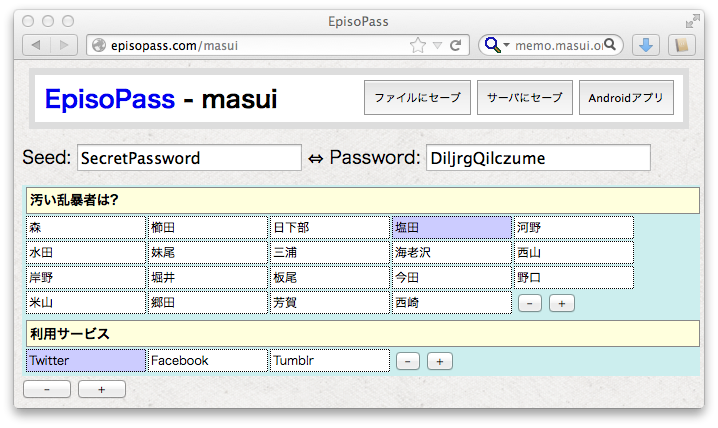
\includegraphics[width=83mm,bb=0 0 718 428]{figures/a9167a6ec6af9c70dd1617e3fc25ec30.png}}
\centerline{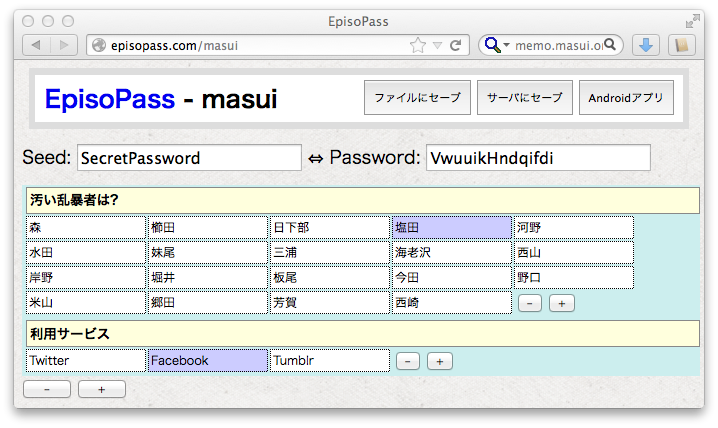
\includegraphics[width=83mm,bb=0 0 718 428]{figures/5b887fabeb8e3319623901fe4a6c56f2.png}}
\caption{サービス名に対応する回答で異なる{\PW}を生成.}
\label{web3}
\end{figure}

定期的に{\PW}変更を求められるシステムでは、
「利用期間は?」という質問に対して
「2013/1」「2013/2」のような答を用意しておけば、
時期を選択することによって簡単に{\PW}を変更することができるので便利である。

\subsubsection{Androidアプリ}

Webサービスを利用する場合、ブラウザとサーバとの間の通信を
記録されたり盗み見されたりされる心配を完全に払拭することはできない。
% 危険を完全になくすことはできない。
前述の例において、
{\PW}はブラウザ内部でJavaScriptにより生成されるので、
一度ページを表示した後は
ネットワークを遮断しても{\PW}計算を行なえるようになっているが、
最初から全く通信を行なわずに{\PW}を作成できる方がより安心であろう。
このため、通信を全く行なわずにマシン単体で{\PW}計算を行なうための
Androidアプリを用意した。
ページの右上の「Androidアプリ」ボタンを押すと、
現在表示している秘密の問題と答を内蔵したAndroidアプリが
サーバ上でビルドされてダウンロードされる。

Android端末でアプリを実行すると図\ref{android1}のような画面が表示される。
{\SS}を設定して「開始」ボタンを押すと図\ref{android2}のように質問がひとつずつ表示され、
ボタンを押してすべて回答すると{\PW}が計算され図\ref{android3}のように表示される。

回答入力と{\PW}計算はAndroid端末で実行されるため、
端末を「機内モード」に設定するなどの方法で
ネットワーク接続を遮断した状態でも{\PW}を計算することができる。
{\EP}をインストールしたAndroid端末を持っていれば常に各種の{\PW}を計算できるので、
他人のマシンや公共の場所に設置されたパソコンなどでも
容易にtwitterなどのネットサービスを利用することができる。

前述の方法で{\EP}アプリをサーバからダウンロードする場合は、
ブラウザ上で秘密の問題をサーバに登録する必要があるが、
秘密の問題を全くネット上に露出することなくアプリを利用することもできる。

\subsection{{\PW}文字列の計算方法}

問題と回答から文字列を生成し、そのMD5値によって{\SS}を換字することにより
{\PW}を生成している。
{\PW}文字列の計算方法は附録に示す。


\section{Discussions}

EpisoPass is just a string-conversion system and it does not
have any information on which candidate is the correct answer.
Also, it does not save any password information at any form, and
it is almost impossible to get the right password 
without having the episodic memory.

\subsection{Advantages of using EpisoPass}

\paragraph{Unforgettable}

%   絶対忘れない
%     30年忘れなかったものは40年忘れないだろう

The biggest advantage of using EpisoPass is that
users don't have to worry about forgetting or losing passwords.
Users of EpisoPass can always save the seed string and question-answer
pairs at any place, and easily generate passwords by answering questions.
If the question is based on old episodic memories,
there is little chance of forgetting correct answers and losing passwords
generated from the selections.
If the episodic memory is based on 20 years ago and the user clearly
remembers it at this moment, it is unlikely that he forgets the episode after
several years.

\paragraph{Usable for everyone}
  
%   老人など、頭が弱くても対応できる

Not everyone is familiar with handling passwords.
Even experienced computer users sometimes use weak passwords,
since choosing a good password is not a straightforward task.
Using EpisoPass, people who cannot create and remember strong passwords
can easily generate strong passwords just by providing secret
questions and answers.
With a good interface, people can even use various password-based
services without noticing the problem of passwords.

% 強いパスワードの作成と記憶が同時にできる

\paragraph{Easy to change passwords}

%   変えるのが簡単
%     問題に「2016」とか「April」とか書いておけばいい

On some systems, users are requested to change passwords periodically
to strenghen security.
A user can generate a new strong password by using a randam character generator
on a PMS, but he might want to old passwords in case some trouble happens.
Using EpisoPass, user can just provide a date-related question-answer pairs,
and generate different strong passwords based on the answer.
(Figure xxx)

\paragraph{All information can be put public}
%   全情報を公開して大丈夫
%     マスターパスワードが要らない
%     秘密裏などは誤って流出する可能性があるが...

\paragraph{Strong passwords can be generated}
%   強度を自由に設定できる

\paragraph{Image-based authentication}
%   画像を使える

Old pictures can be used as the questions of EpisoPass.
Even when people cannot create good secret questions,
people can fairly easily select a secret image from their photo collections
and use it as the question.
For example, if you have a n old picture of your friend,
you can use it as the question
and use his real name and other similar names as candidate answers.

例をここでいろいろ出す

% 画像検索とかされないようにする必要はある

Of course, the photo should not have information related to the
person's real name, since image search is fiarly easy on the Web these days.

\paragraph{Simple implementation}
%   実装が簡単

The algorithm of generating a password is quite simple and
it can be implemented on any browser JavaScripts or
applications on smartphones and small devices.

\paragraph{パスワード自体の漏洩の心配が不要}
% 聞かれてもわからないし書き留める必要がないからウッカリもらす可能性はない
% ローカルに実行すればネットでもれる心配もない

Since the password is generated by the algorithm and the password
string is not kept on a computer in any form,
unexpected leak of the password is unlikely.
The user doesn't have to remember the string and
there is no chance he will reveal it to somebody
even when he is forced to tell the password.

% そのためにAndroidアプリも用意した

\subsection{Risks of using EpisoPass}

\paragraph{Security strength of EpisoPass}
% ■ 安全性

{\PW}は長年利用されているため
強度や実際の運用に関して多くの研究が存在するが%
\cite{Hayashi:2011:DSP:1978942.1979326}%
\cite{Komanduri:2011:PPM:1978942.1979321}% どういうパスワードが強いか
、{\SQ}の強度に関しては充分研究されていない。
{\EP}の運用実績は長くないが安全性などについて考察を行なう。

{\EP}で
選択枝が10個の{\SQ}を8個使用する場合、
総当たりで{\PW}を生成するには
1億($10^8$)通りの試行が必要であり、
% エントロピーは26.6 ($ = 8 \times \log_2 10$) ビット
エントロピーは26.6ビットとなる。
英字からランダムに8文字を並べて作成した{\PW}のエントロピーは37.6ビットになるが、
``\textsf{pmvixuzq}''のように全く意味のない{\PW}を記憶して利用することは少ないため、
実際に利用される{\PW}のエントロピーは20ビット程度と考えられているので\cite{NIST}、
{\SQ}と選択枝の数を10個程度用意すれば
通常の{\PW}と同程度の強度が期待できることになる。
%
総当たり攻撃が可能なオフライン運用ではエントロピーの大きさは重要であるが、
オンラインサービスでは
{\PW}入力を何度か間違えるとサービスがブロックされるのが普通なので、
それほど長い{\PW}を用意する必要は無いと考えられている\cite{Florencio:2007:SWP:1361419.1361429}。

一方、{\SQ}を利用する認証の脆弱性を利用した攻撃が近年問題になっている。
{\PW}を忘れたときのために、
あらかじめ設定した{\SQ}に答えることによって{\PW}をリセットできるサービスがあり、
「母親の旧姓は?」や「最初に飼ったペットの名前は?」のような
質問に対してユーザが答を登録するようになっている。
このような問題は他人が調べたり推測したりすることが容易であるうえに
{\SQ}の数は一般的に少なく、
{\PW}よりも脆弱だといえる\cite{Rabkin:2008:PKQ:1408664.1408667}。% 銀行20個調べて{\SQ}の弱さを指摘
%
ユーザが作成した{\SQ}を使えばこのような問題はなくなるはずであるが、
他人に解かれにくい問題をユーザが作成することは難しく、
またユーザ自身が答を忘れてしまうことも多いと考えられている\cite{Just:2009:PCC:1572532.1572543}\cite{Schechter:2009:NSM:1607723.1608145}。
%
また、古い記憶にもとづいて作成した秘密の問題は
ユーザが想像するよりも解かれやすいという実験結果にもとづき、
忘れない{\SQ}を複数利用する方法、
問題と答を連想するために画像を利用する方法、
複数の問題を連続的に利用する手法などが提案されている\cite{Renaud:2010:PQE:2146303.2146318}。

{\EP}では、
他人には解くことが難しく自分では忘れないような{\SQ}を自由にいくつでも利用できるようになっている。
問題作成に慣れていないユーザには有効な{\SQ}を作成することは難しいかもしれないが、
次節で述べるように、適切な質問を選ぶことによりこの問題を解決できるはずである。

The strength of the generated password depends on the number of
questions and the 'secretness' of the questions.
If the episodic memory is shared by someone else,
that personn can easily answer the question and generate the
password just like the user.

Questions like "Which one is your favorite?" should be avoided,
since some of the friends might know the user's taste.
Questions related to a episode which the user is proud of should also be
avoided, since the user might talk aboutu the episode to somebody else.



If, one of the passwords generated by EpisoPass is revealed
for some reason,... フルートフォースでとかれる可能性はある

To prevent such troble, it is safer to keep all the q-a pairs secret.

問題を時々変えるのが安全だろう

問題自体が秘密であればひとつ漏れても大丈夫

\subsection{問題の選択}

{\EP}利用において{\SQ}の選択は非常に重要である。
他人が推測することが難しく、自分が決して忘れないような{\EM}を{\SQ}として利用すべきであり、
以下のような性質をもつ記憶は{\SQ}として利用すべきではない。

\begin{itemize}
\item \textsf{自慢になるもの
(何かの機会にうっかり他人に話してしまう可能性がある)}

\vspace{-1mm}
\item \textsf{ネット上に記録が残っているもの}

\vspace{-1mm}
\item \textsf{他人と情報を共有しているもの}

\vspace{-1mm}
\item \textsf{趣味や嗜好に関連するもの
(他人に推測されやすいうえに嗜好が変化する可能性がある)}

\end{itemize}

\noindent
このようなものではなく、
「わざわざ人に話すことはないが自分の記憶に強く残っているような無難な{\EM}」を
{\SQ}として利用するのが良いであろう。
具体例としては以下のようなものがある。

\begin{itemize}
\item 昔のちょっとした怪我の場所や種類

\vspace{-1mm}
\item 昔のちょっと悔しい思い出

\vspace{-1mm}
\item 昔何かを見つけた場所
\end{itemize}

たとえば図\ref{kega}のような{\SQ}は他人に話したことが無いが、
痛い思いをしたことは忘れないし、
偽答を作成するのも簡単なので、
認証のための{\SQ}として適切であると考えられる。

\subsection{偽答の作成方法}

{\SQ}の種類によっては偽答の生成が難しい場合がある。
図\ref{atmega}は電子工作に関する{\SQ}の例であるが、
正答と区別がつかない偽答を充分リストすることは難しい。

\begin{figure}[H]
\centerline{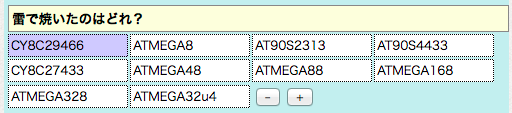
\includegraphics[width=83mm,bb=0 0 512 113]{figures/2f63ceb9ab6faf8d81393953f2f95a8c.png}}
\caption{偽答の生成が難しい例.}
\label{atmega}
\end{figure}

一方、正答として人名や地名を利用する場合、
正答に似た人名や地名をリストすることは難しくない。
「世田谷」が正答であるとき、
「目黒」「杉並」のような偽答を用意するのは簡単である。
%
正答と同じカテゴリに属する単語を自動的にリストすることができれば
正答をもとにして簡単に偽答のリストを生成することができる。
%
ひとつの単語もしくは単語の集合と同じカテゴリに属する単語を検索する手法は
「同位語検索」と呼ばれ、
Webのデータを利用した様々な同位語検索システムが提案されている%
\cite{Huang:2012:LFC:2426725.2426728}% 読んでないけど
\cite{BooWa}% Boo!Wa!というサイトをやっている
\cite{Wang:2007:LSE:1441428.1442086}% BooWa
\cite{大島裕明:2006-12-15}% ライバルサーチ「やーやら」
。
たとえば「ライバルサーチ『やーやら』」\cite{大島裕明:2006-12-15}は、
Web上の「AやBが」のような表現を抽出することによって
AとBのカテゴリが近いことを判断している。

人名や地名の偽答を作成したい場合は
人名や地名のデータベースを利用して偽答を生成することができる。
市町村の人口ランキングや位置関係のデータなどを利用すれば
似た地名を偽答としてリストすることが可能であるし、
人名ランキングを利用すれば
似た苗字を偽答とすることができる。
たとえば日本の名字ランキングの40位近辺に
「長谷川」「近藤」「石井」「斉藤」「坂本」「遠藤」「藤井」
などの名字があるので、
「石井」が正答のときこれらの名字を偽答にすればよい。
しかし、
「小学生のとき〜だった同級生は誰?」という{\SQ}の正答が「石井」であるとき
この方法で偽答を生成すると、
「長谷川」「近藤」などの同級生の存在を確認することにより
正答が「石井」であることが判明してしまう可能性があるので注意が必要である。

\subsection{{\PW}漏洩時の問題}

{\SQ}を公開している場合、
{\SS}と{\PW}の対応がひとつでも漏洩してしまうと、
総当たり計算でチェックすることにより、
すべて{\SQ}の正答が判明してしまう。
{\SQ}の正答を知っていれば
{\SS}から{\PW}を計算することができるので、
漏洩した{\SQ}は利用不可能になってしまう。
%
\ref{pattern1}や
\ref{pattern2}のような運用をしている場合は
{\PW}がひとつ漏洩しても他の{\PW}は安全だが、
\ref{pattern3}のような運用をしている場合は
ひとつでも{\PW}が漏洩するとあらゆる{\PW}が漏洩してしまうことになる。

\subsection{画像認証の利用}

忘れにくい{\EM}を利用する認証手法として
様々な画像認証システム\cite{Biddle:2012:GPL:2333112.2333114}\cite{GraphicalPasswords}\cite{小池英樹:2006-05-15}が提案されている。
複数の画像の中から正答を選択するもの(Cognometric方式)、
ひとつの画像の中の特定の場所を指定するもの(Locimetric方式)、
画像の上で描画操作を行なうもの(Drawmetric方式)
が広く利用されているが\cite{Biddle:2012:GPL:2333112.2333114}\cite{GraphicalPasswords}\cite{Guideline}、
{\EP}は図\ref{web1}のように
文字列のかわりに画像URLを{\SQ}として利用する点が異なっている。
%
Cognometric方式は{\EM}を効果的に利用できるが、
多数の偽答画像が必要だという問題がある。
Locimetric方式は
{\EM}を効果的に利用できないことに加え、
クリックしやすい「ホットスポット」は限られているため
充分なエントロピーを確保できないことが問題になる\cite{Dirik:2007:MUC:1280680.1280684}。
またDrawmetric方式も{\EM}を効果的に利用できないし、
ユーザは似た傾向のストロークを選びがちであるため
充分なエントロピーを確保しにくいことが知られている\cite{Nali}。
%
{\EP}のように画像を{\SQ}として利用する場合、
通常の{\SQ}の場合と同様に偽答を増やすことが容易であることに加え、
画像に関連した{\EM}を有効に利用できるという利点がある\cite{増井:CSS}。

図\ref{leiko}は
本棚.org\cite{hondana}\cite{hondanaorg}
のユーザのひとり\footnote{
  \textsf{http://hondana.org/Leiko}
}が利用している画像認証問題である。
このユーザ以外には正答は見当もつかないが、
本人にとっては忘れることがない{\EM}と結びついた画像だということであった。


% 答を書くわけではないから安全
% 心配ならオフラインでやれば大丈夫
% 
% 弱いパスワードを強くすることも簡単
% 
% 
% Bookmarkletも用意した
%   拡張機能も用意したい
%

\section{Related Work}

認証手法は本当に沢山あり、パスワードを置き換えようとするものも多いが
まだ成功はしていない

パスワード管理システムは充分広く使われている

% A Password Manager that Doesn’t Remember Passwords
\cite{Stobert:2014:PMD:2683467.2683471} % Visipass 画像クルーからパスワード生成

% 様々なシステムがあるが、エピソード記憶からパスワードを直接生成するものは無い
% 
% パスワード管理システム
%   沢山ある
% 
% 強いパスワードを作るシステム
%   ランダムに生成するサイトが沢山ある
% 
% 強いパスワードを覚えるための工夫
%   Bonneau
% 
% 画像を使う
% 
% パスワードに関する全情報を公開してどこかに置いておける
%   ググれるかもしれない
%   紛失する可能性が少ない
%

\section{Experiences}
% ■ 運用実績

\section{Limitations}

% なぞなぞ問題を考えるのが難しい
%   自分だけ知ってる秘密など思いつかない人が多い
%   しかしインタビューを行なうとそういうのは出てくる
%     子供のときの怪我、ケンカ、失敗など
%     特に、自慢にならないものが良い
% 
% 強度が直感的でない
%   誰でも簡単にとけるのじゃないかと思う
%   safe感覚が足りない

\section{CONCLUSION}

{\EM}に結びついた{\SQ}を利用して{\PW}を生成/管理できるシステム{\EP}を提案した。
{\EP}は単純な原理にもとづいており柔軟な利用形態が可能であり、
強力な{\SQ}を用意することにより
秘密情報を全く覚えることなく安全な認証を行なうことができる。
%
強力な{\SQ}を作成して安全に運用が可能かどうかを長期的に評価したいと考えている。
%
%欠点:
%なぞなぞを考えるのがめんどくさい
%安全になぞなぞを扱うのが面倒
%  ネットなしで運用したりとか
%運用を間違うと思わぬところで回答がバレる可能性がある
%
{\EP}は\textsf{http://Episopass.com/}で運用しており、
ソースはGitHubで公開している\footnote{
  \textsf{http://GitHub.com/masui/EpisoPass}
}。

{\scriptsize
\bibliographystyle{acm-sigchi}
\bibliography{paper}
}

\section*{Appendix: Algorithm for generationg a password}

% {\PW}は、
% {\SQ}と回答の組合せにもとづいて{\SS}を換字することによって計算される。
% 換字は文字種ごとに行なわれる。
% たとえば
% {\SS}の1桁目が数字のときは{\PW}の1桁目は数字に変換され、
% {\SS}の1桁目が記号のときは{\PW}の1桁目は記号に変換される。

% https://ja.wikipedia.org/wiki/換字式暗号

The password string is generated by
substituting the characters in the seed string
based on the user's selections of candidate answers.
Character substitution is performed based on the chracter types.
For example, if the first character of the seed string is a digit,
the first character of the generated password string is also a digit.

% {\SS}内の数字$A$は、換字関数$f_N()$によって{\PW}内の数字$B$に変換される。
% $f_N()$ は以下のような関数である。

A digit $A$ in the seed string is converted to a digit $B$
in the password string by the following
character substitution function $f_N()$.

\[ f_N(x) = (10 + N - x) \bmod 10 \]

% ここで$N$は{\SS}と回答の組み合わせから計算される自然数で、
% 答の選択により変化する。
% たとえば$N = 5$ のとき、$f_5(x) = (15-x) \bmod 10$ となるので、
% $x$と$f_5(x)$の対応は以下のようになる。

Here, $N$ is a number calculated from the user's selection of
candidate answers.
If the value of $N$ if $5$, $f_5(x) = (15-x) \bmod 10$, and
$x$と$f_5(x)$の対応は以下のようになる。

\[ f_5(0) = 5 \]
\[ f_5(1) = 4 \]
\[ f_5(2) = 3 \]
\[ ... \]
\[ f_5(8) = 7 \]
\[ f_5(9) = 6 \]

% $f_N()$は$N$により変化するので、$N$がわからなければ$f_N()$もわからない。
% $N$は{\SS}と回答の組み合わせから計算される自然数なので、
% {\SS}の答を知らなければ$N$を計算することはできず、
% 問題と答の組み合わせを知らない限り{\SS}から{\PW}を計算することはできない。

$f_N()$ depends on the value of $N$, and
it is impossible to know about $f_N()$ without knowing the value of $N$.
 
% {\EP}では以下のようにして$f_N()$を計算している。

$N$ is calculated by the following algorithm in EpisoPass.
 
\begin{enumerate}
  % \item 問題文字列と選択した答の文字列の組を連結して長い文字列$S$を生成
  \item Generate a string $S$ by concatinating all the question strings and selected candidate answers.

    \vspace{-1mm}
  % \item $S$のMD5ハッシュ値$M$(16進32桁の文字列)を計算
  \item Calculate the MD5 value of $S$ and generate 32-byte hexadecimal string $M$.

    \vspace{-1mm}
  %\item {\SS}の$k$桁目の文字に対し、
  %  $M$の$k \times 4$文字目から$k \times 4 + 3$文字目までの部分文字列(16進4桁)を取得し、
  %  それを$N$とする
  \item For each $k$th chracter of {\SS},
    get the 4-character substring of $M$ beginning at $k \times 4$, and use it as the value of $N$

    %たとえばハッシュ値$M$が$12345678...$だったとき、1桁目を計算する$f()$についてはN=0x1234となる。
    If the hash value $M$ is $12345678...$,
    $f_0x1234$ is used as the substitution function for the first character,
    $f_0x5678$ is used as the substitution function for the secound character, etc.
\end{enumerate}

\end{document}

* このサービスが終了したらネットライフが終了する
* 増井さんが飽きてサービス止めちゃったら多くの道連れがでるという罠

=> EpisoPassのHTMLやAndroidアプリを持っていればEpisoPass.comが無くても計算可能です。
アルゴリズムは単純ですし公開されているわけですから別実装してもいいでしょう。

* いまいちよくわからないです。seed というのもおぼえてないといけないのでしょうか?

=> Seedは覚えておいてもいいですし公開してもかまいません。私は全部公開しています。

* 使うのちょっとめんどくさそう

=> パスワード入力のたびに使うわけではありませんし、問題に答えるのにそれほど
時間はかかりません。新しくスマホを買ったら使うぐらいです。
問題を作るのは確かにめんどくさいかもしれません。

* 秘密の質問に入れる偽装の答えをどこにメモしたか忘れるという事もしばしば

=> 問題も答も公開しておけば忘れることはないでしょう。

* クイズにできるエピソードがない人はどうすればいいんでしょう

=> そういう話はよく聞くのですがエピソードが無い人なんているのでしょうかね?
小学校のときちょっとしたケガ体験とかエピソードとか覚えてませんか?

* EpisoPassのフィッシングサイトができたらどうしましょう

=> 完全にローカルHTMLかローカルアプリで使えば安心でしょう。

* URLがseed込みなので、ブックマークつくっておけば辿りつける、という主張だったかと

=> これは誤解です。URLは計算には関係ありません。

* Q:(1)seedはどうやって作るのか?(2)質問はどうやって作るのか?

=> (1) Seedはなんでもいいです (2) 質問は頑張って作ります

* 親しい人が協力すると突破できるなあ

=> それは問題次第です。私が公開してるものは無理だと思います。
汚い乱暴者は誰でしょう? ケガした町名は?

* これは本当に使ってみたいんだけど、ちょっと勇気いるんですよね。

=> 勇気は確かに必要だと思います...

* 同じ旅行に行った人だけが分かるエピソードをパスにして、写真共有とかいけますかね

=> 複数の人間で秘密を共有できますし認証の強度も自由に制御できます

* 増井さんのパスワードの質問と解答、誰でも自由に書き換え可能なように見えるんですが、こういう仕様?

=> そうです。編集に認証入れたくないですので。確かに消されたりする問題はあるのですが
ローカルに問題をセーブしておけば大丈夫です。

* 僕はEpisoPassを使っていて、「好きな○○は?」という質問を作ったら、正解が変質して、正解が生成出来なくなったことがありますね。

=> 絶対忘れない事実を問題として登録しておけばいいでしょう。好みは変わる可能性があるので問題として適切ではありません。

* Seedと問題を全部公開できるのは素晴らしい発想ですが、Passwordが
一個でもばれると、残りが全部ばれるのは何とかできないですかね。。。
一つばれるとヤバイ、という点では同一パスワードの使いまわしと原理的に同じ?

=> 問題を全部変えればいいんですが難しいですね... これは対策を考えたいと思います。
しかしそもそもパスワード流出させるサービスの存在がアウトオブ論外なわけですが...

* あれ、問題を増やしたら、過去に登録したパスワードを全部変えなければ
ならなくなる、ということでしょうか?

=> 過去に登録したパスワード計算には過去の問題を使い、新しく登録したいパスワードは
新しい問題を使えばいいかもしれません。あらゆるパスワード生成に同じ問題を
使う必要はありませんので。